\documentclass{beamer}
\usetheme{Boadilla} 
\usecolortheme{whale}
%Choix du thème de la police (sans serif, petites capitales dans les titres...) 
\usepackage{amssymb} 
% Des symboles mathématiques
\usepackage{graphicx}
% Pour insérer des images
\usepackage{multicol}
% Pour gérer facilement un environnement à n colonnes
\usepackage{booktabs}
% Pour des beaux tableaux
\usepackage{esvect} 
% Pour de belles flèches sur les vecteurs
\usepackage{esdiff}
% Pour de beaux symboles de dérivation
\usepackage{siunitx}
% Pour l'utilisation des unités du système international
\sisetup{output-decimal-marker={,},inter-unit-product=\ensuremath{{}\cdot{}}}
% Quelques réglages pour l'affichage des unités

% Pour les couleurs
\usepackage{color}
% Pour les indentations
\usepackage{tcolorbox}
\tcbuselibrary{skins, breakable}
\newtcolorbox{indentation}[1][]{
	blanker, left=1cm, borderline west={0.5mm}{0.6cm}{black!50}, breakable,
	before skip=2ex plus 0.1ex, after skip=2ex plus 0.1ex, #1
}
% Commande pour utiliser une indentation :
% \begin{indentation}
%     <texte>
% \end{indentation}

% Pour écrire du code en Python :
\usepackage[utf8]{inputenc}
\usepackage[T1]{fontenc}
\usepackage{xcolor}
\usepackage{listings}

\lstset{%
  language=Python,
  basicstyle   = \ttfamily\tiny,
  keywordstyle =    \color{orange},
  keywordstyle = [2]\color{blue},
  commentstyle =    \color{gray}\itshape,
  stringstyle  = \color{green!50!black},
  numberstyle = \color{gray},
  numbers = left,
  frame = single,
  framesep = 2pt,
  breaklines = true,
  aboveskip = 1ex,
  xleftmargin = 8mm,
  framexleftmargin = 8mm,
  literate        =
                        {é}{{\'e}}{1}%
                        {è}{{\`e}}{1}%
                        {à}{{\`a}}{1}%
                        {â}{{\^a}}{1}%%%
                        {ç}{{\c{c}}}{1}%
                        {œ}{{\oe}}{1}%
                        {ù}{{\`u}}{1}%
                        {É}{{\'E}}{1}%
                        {È}{{\`E}}{1}%
                        {À}{{\`A}}{1}%
                        {Ç}{{\c{C}}}{1}%
                        {Œ}{{\OE}}{1}%
                        {Ê}{{\^E}}{1}%
                        {ê}{{\^e}}{1}%
                        {î}{{\^i}}{1}%
                        {ï}{{\"i}}{1}%%%
                        {ô}{{\^o}}{1}%
                        {û}{{\^u}}{1}%
}

\title[]{Sécurisation des échanges d'informations entre deux ordinateurs}
\author{Maxime LE BLAN}
\date{28798}

\begin{document}

\begin{frame}
  \titlepage 
%Génère une page avec les données fournies précédemment.
\end{frame}

\begin{frame}{Système d'étude}
\begin{figure}[H]
  \centering
  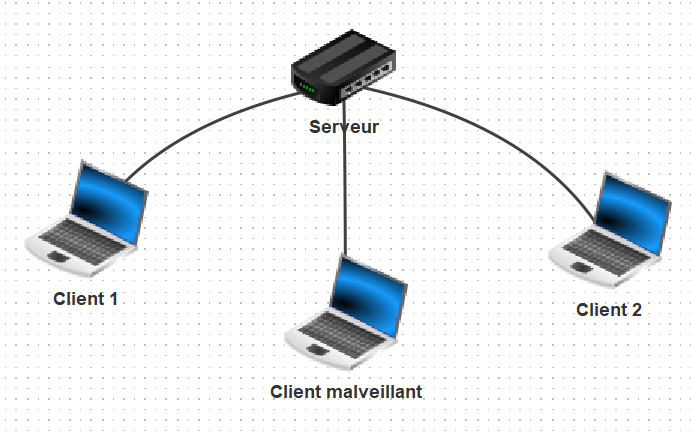
\includegraphics[scale=0.5]{reseau_2.png}
  \caption{Representation imagée du système étudié}   
  \label{fig:reseau_2}
\end{figure}
\end{frame}

% PBQ :
% Comment garantir au mieux la sécurité et l’efficacité des échanges d’informations entre deux ordinateurs en nous basant sur des algorithmes existants ?

\begin{frame}{Sommaire}
\tableofcontents[sections={1-5}]
\end{frame}

\section{Définitions des notions et méthodes d'implémentations}
\begin{frame}{Vocabulaire}
\begin{figure}[H]
  \centering
  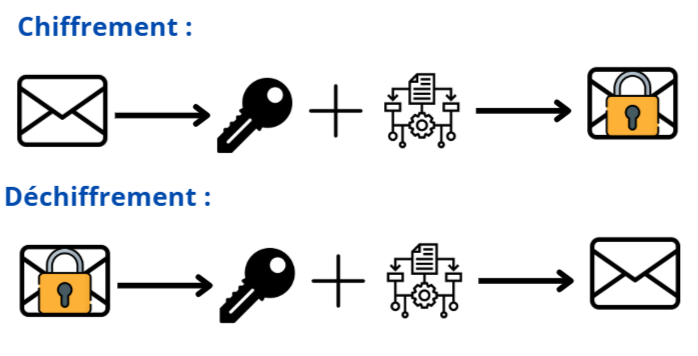
\includegraphics[scale=0.5]{defs.png}
\end{figure}    
\end{frame}

\begin{frame}{Définitions}
\begin{figure}[H]
  \centering
  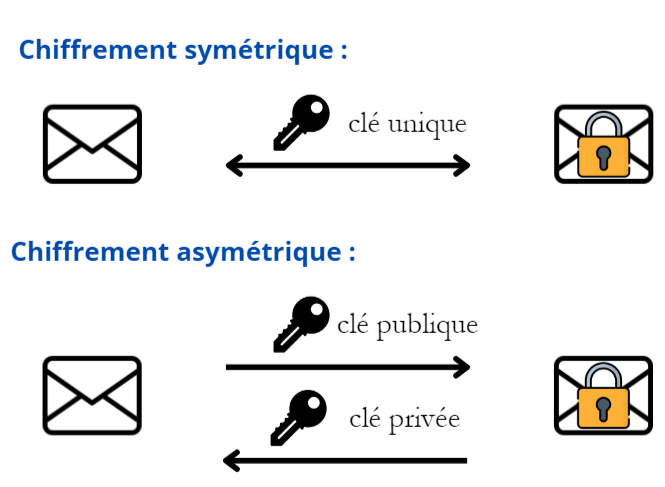
\includegraphics[scale=0.6]{def_cles.png} 
  \label{fig:def_cles}
\end{figure}
\end{frame}

\begin{frame}{Implémentation}
\begin{figure}[H]
  \centering
  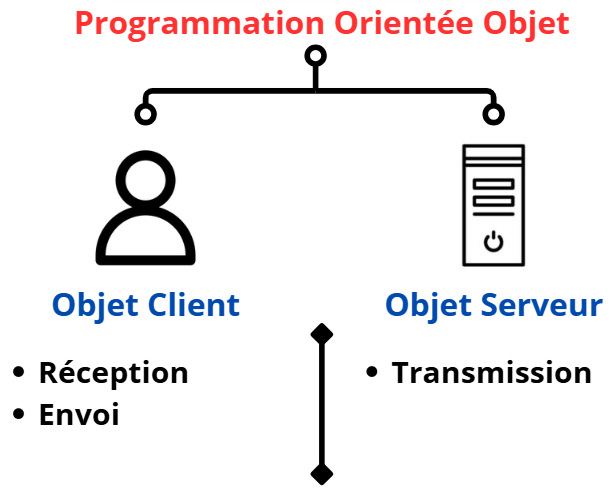
\includegraphics[scale=0.5]{poo_1.png}
  \label{fig:poo_1}
\end{figure}
\end{frame}

\begin{frame}{Implémentation}
\begin{enumerate}
    \item Problèmes :
    \begin{itemize}
        \item Programmation séquentielle ne permet pas d'envoyer et de recevoir des messages en même temps
        \item Envoie de données multiples ne peut se faire qu'avec des chaines de caractères
    \end{itemize}
    \item Solutions :
    \begin{itemize}
        \item Utilisation de fils d'exécutions
        \item Fonctions de conversion de liste de données chiffrées en chaines de caractères
    \end{itemize}
\end{enumerate}
\end{frame}

\section{Premier modèle de sécurisation avec l'algorithme RSA}
\begin{frame}{Algorithme RSA}
\begin{enumerate}
    \item Algorithme de chiffrement asymétrique
    \item Se base sur deux conjectures :
    \begin{itemize}
        \item "casser" RSA par force brute nécessite de trouver la décomposition en facteurs premiers d'un nombre entier de grande taille
        \item les algorithmes existants ont une complexité exponentielle en la taille de la clé
    \end{itemize}
\end{enumerate}
\end{frame}

\begin{frame}{Exemple}
\begin{figure}[H]
  \centering
  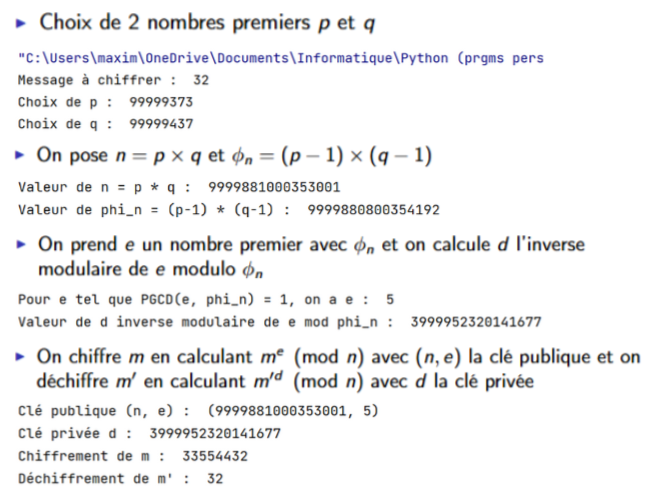
\includegraphics[scale=0.5]{ex_rsa_3.png}
  \caption{Exécution de l'algorithme RSA sur un exemple}
  \label{fig:ex_rsa_3}
\end{figure}
\end{frame}

\begin{frame}{Protocole du modèle n°1}
\begin{figure}[H]
  \centering
  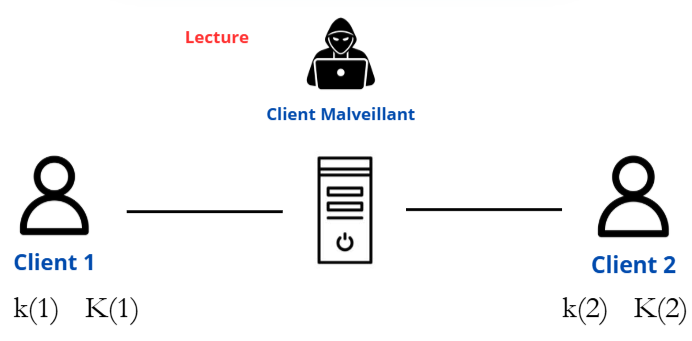
\includegraphics[scale=0.5]{rsa_1.png}
  \caption{Les clients échangent leur clé publique $K$ respective}
  \label{fig:p_rsa_1}
\end{figure}
\end{frame}

\begin{frame}{Protocole du modèle n°1}
\begin{figure}[H]
  \centering
  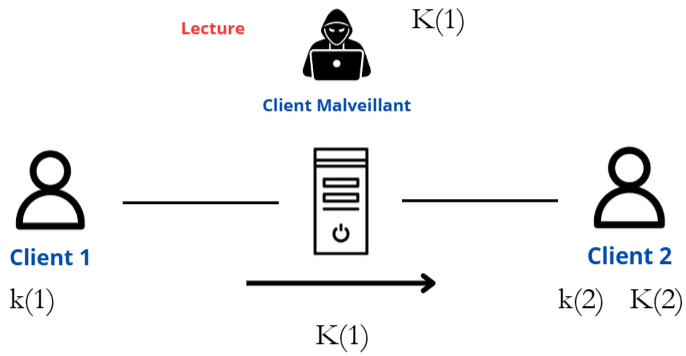
\includegraphics[scale=0.5]{rsa_2.png}
  \caption{Le client 1 envoie sa clé publique $K(1)$ au client 2 en passant par le serveur}
  \label{fig:p_rsa_2}
\end{figure}
\end{frame}

\begin{frame}{Protocole du modèle n°1}
\begin{figure}[H]
  \centering
  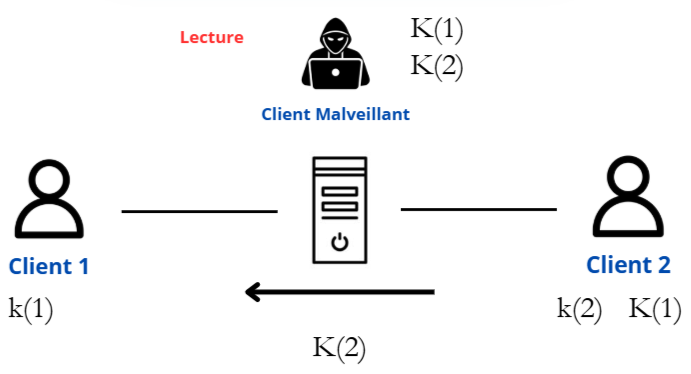
\includegraphics[scale=0.5]{rsa_3.png}
  \caption{Le client 2 envoie en retour sa clé publique $K(2)$ au client 1 en passant par le serveur}
  \label{fig:p_rsa_3}
\end{figure}
\end{frame}

\begin{frame}{Protocole du modèle n°1}
\begin{figure}[H]
  \centering
  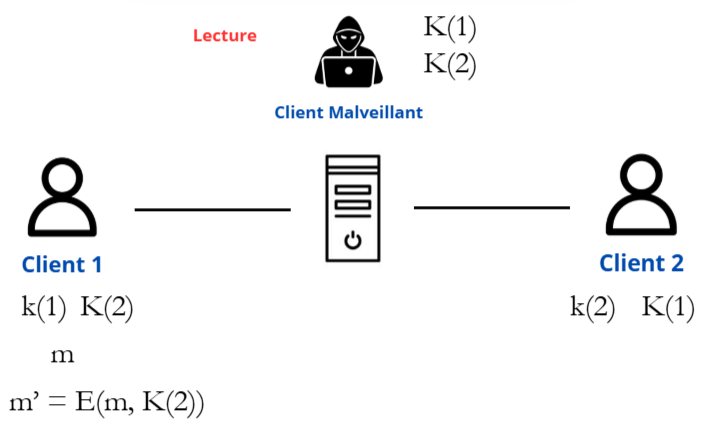
\includegraphics[scale=0.5]{rsa_4.png}
  \caption{Le client 1 chiffre le message $m$ avec la clé $K(2)$ et la fonction de chiffrement $E$}
  \label{fig:p_rsa_4}
\end{figure}
\end{frame}

\begin{frame}{Protocole du modèle n°1}
\begin{figure}[H]
  \centering
  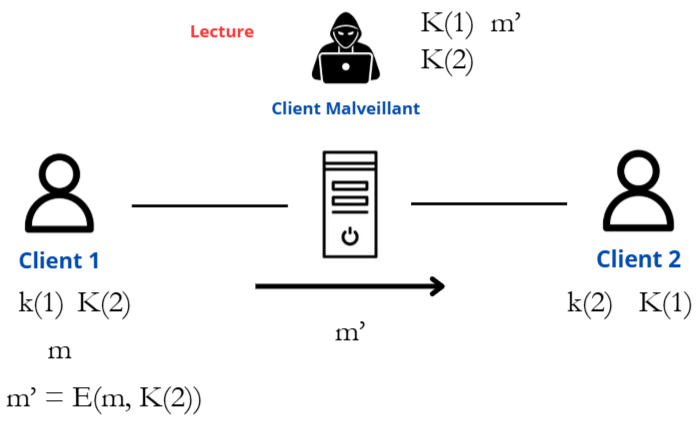
\includegraphics[scale=0.5]{rsa_5.png}
  \caption{Le client 1 envoie le message chiffré $m'$ au client 2 en passant par le serveur}
  \label{fig:p_rsa_5}
\end{figure}
\end{frame}

\begin{frame}{Protocole du modèle n°1}
\begin{figure}[H]
  \centering
  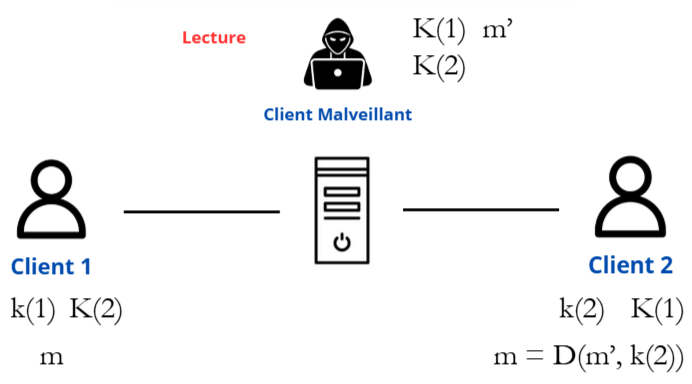
\includegraphics[scale=0.5]{rsa_6.png}
  \caption{Le client 2 reçoit $m'$ et le déchiffre avec sa clé privée $k(2)$ et la fonction de déchiffrement $D$}
  \label{fig:p_rsa_6}
\end{figure}
\end{frame}

\begin{frame}{Test pratique}
\begin{figure}[H]
  \centering
  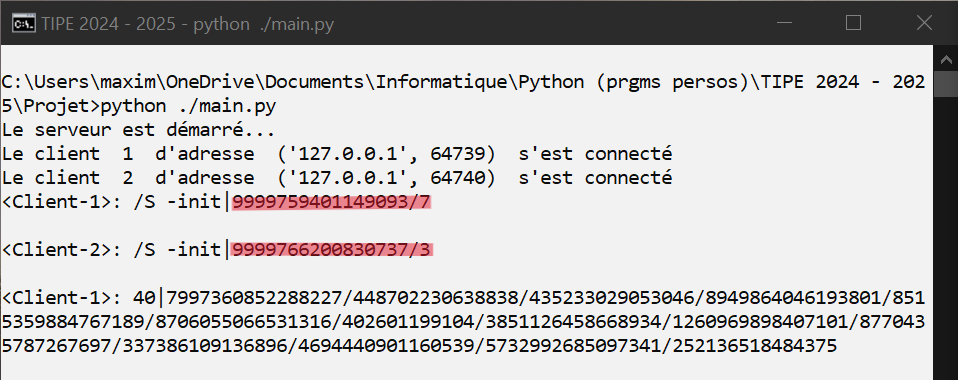
\includegraphics[scale=0.5]{cmd_rsa_1a.png}
  \caption{Visuel du transit du message chiffré 'Message secret ecrit par Maxime LE BLAN' par le serveur, et de ce que peut voir le client malveillant}
  \label{fig:cmd_rsa_1a}
\end{figure}
\end{frame}

\begin{frame}{Test pratique}
\begin{figure}[H]
  \centering
  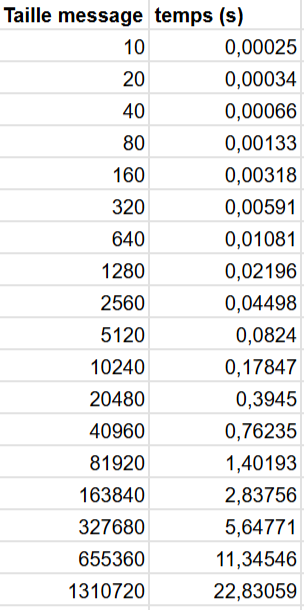
\includegraphics[scale=0.42]{tab_rsa.png}
  \caption{Temps écoulé entre l'envoi et la réception d'un message en fonction de la taille de celui-ci avec RSA}
  \label{fig:tab_rsa}
\end{figure}
\end{frame}

\begin{frame}{Efficacité de l'algorithme RSA}
\begin{minipage}[c]{0.30\linewidth}
    \textbf{Remarque :} La complexité temporelle de l'algorithme RSA est en $O(m)$ avec $m$ l'équivalent entier du message littéral
\end{minipage}
\begin{minipage}[c]{0.40\linewidth}
    \begin{center}
      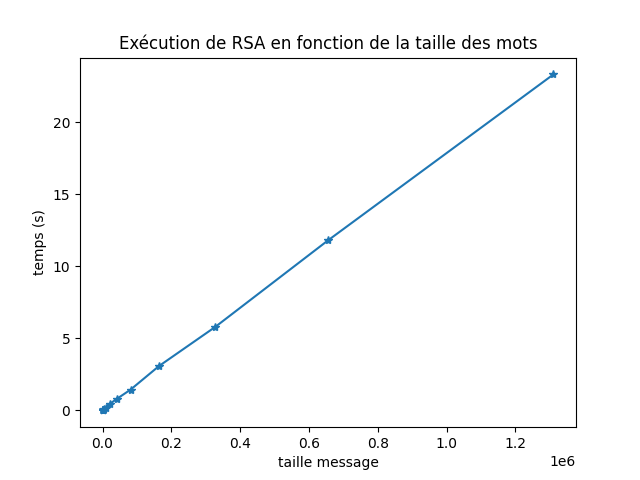
\includegraphics[scale=0.5]{graphe_rsa.png}
    \end{center}
\end{minipage}
\end{frame}

\section{Amélioration du premier modèle avec l'algorithme AES}
\begin{frame}{Algorithme AES}
    \begin{center}
      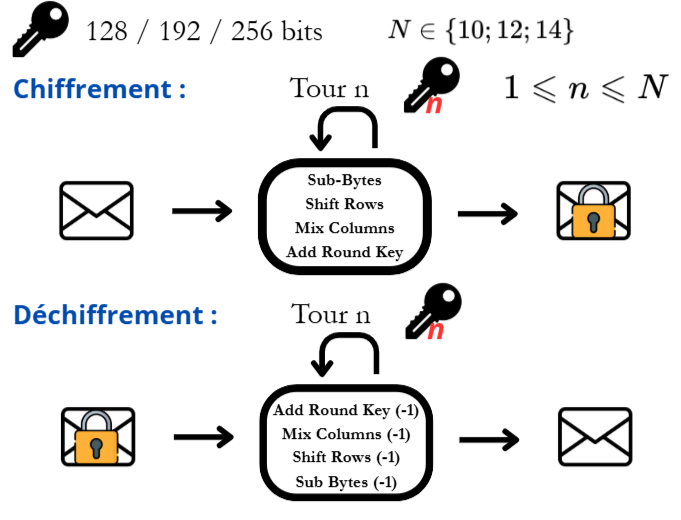
\includegraphics[scale=0.58]{algo_aes.png}
    \end{center}
\end{frame}

\begin{frame}{Exemple avec Sub-Bytes et Shift Rows}
    \begin{center}
      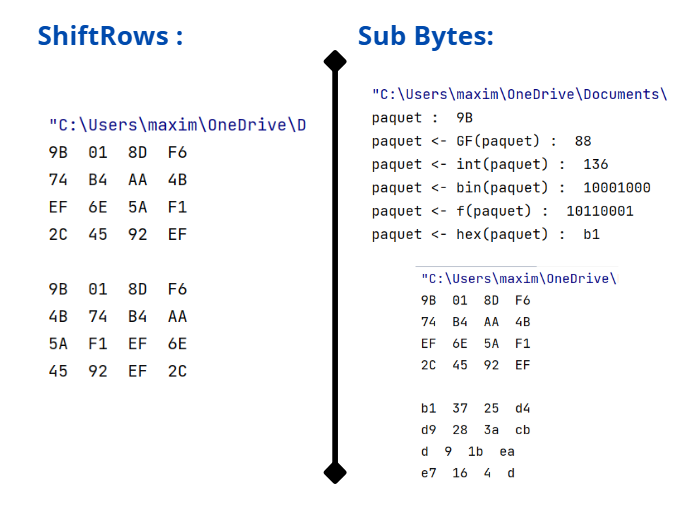
\includegraphics[scale=0.58]{aes_exemple.png}
    \end{center}
\end{frame}

\begin{frame}{Protocole du modèle n°2}
\begin{figure}[H]
  \centering
  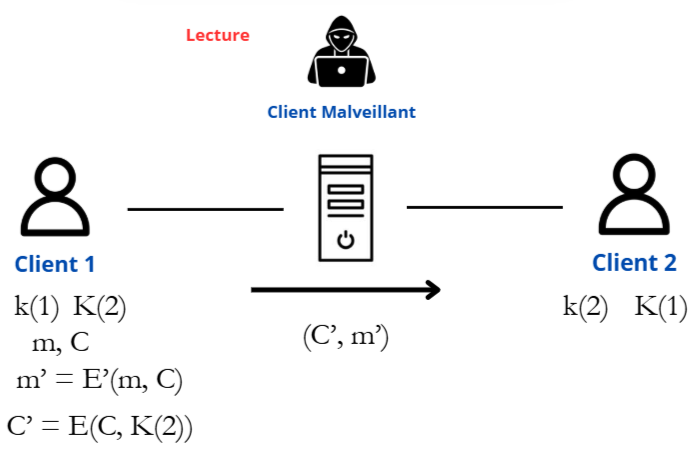
\includegraphics[scale=0.5]{aes_1.png}
  \caption{Cette fois-ci, $m$ est chiffré avec la clé $C$ de AES puis $C$ est chiffrée avec $K(2)$}
  \label{fig:p_aes_1}
\end{figure}
\end{frame}

\begin{frame}{Protocole du modèle n°2}
\begin{figure}[H]
  \centering
  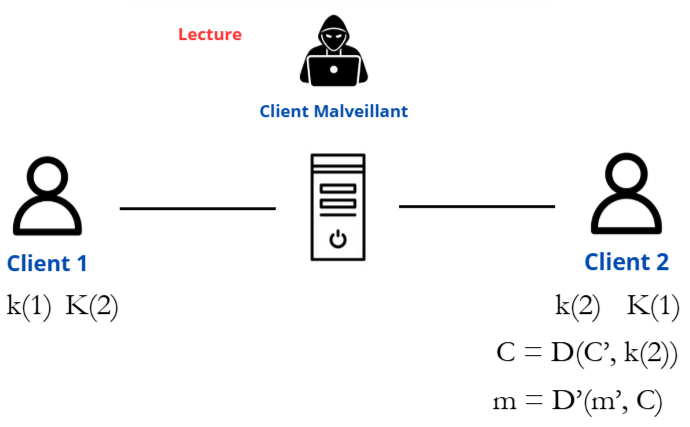
\includegraphics[scale=0.5]{aes_2.png}
  \label{fig:p_aes_2}
\end{figure}
\end{frame}

\begin{frame}{Test pratique}
\begin{figure}[H]
  \centering
  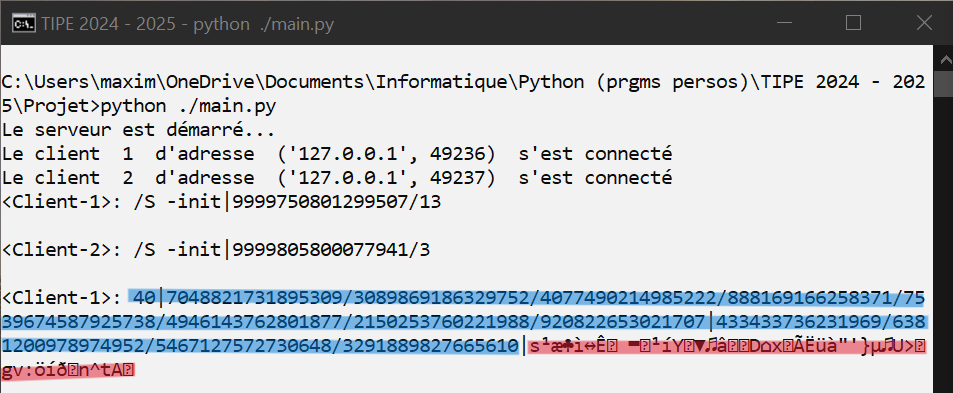
\includegraphics[scale=0.5]{cmd_aes_1a.png}
  \caption{Visuel du transit du message chiffré 'Message secret ecrit par Maxime LE BLAN' par le serveur, et de ce que peut voir le client malveillant}
  \label{fig:cmd_aes_1a}
\end{figure}
\end{frame}

\begin{frame}{Test pratique}
\begin{figure}[H]
  \centering
  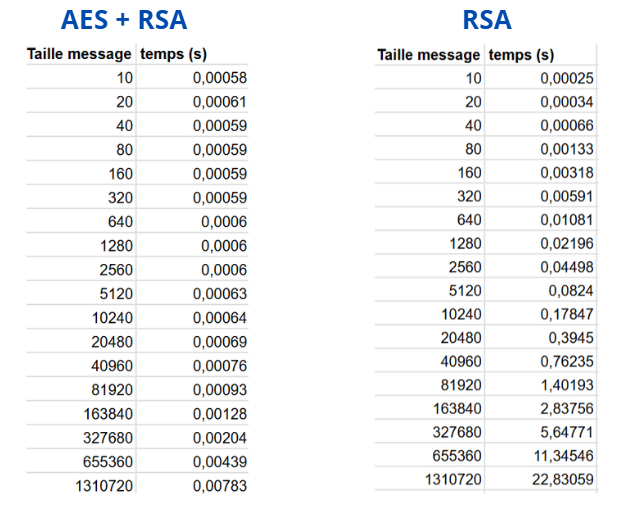
\includegraphics[scale=0.47]{tab_comp_aes_rsa.png}
  \caption{Temps écoulé entre l'envoi et la réception d'un message en fonction de la taille de celui-ci}
  \label{fig:tab_comp_aes_rsa}
\end{figure}
\end{frame}

\begin{frame}{Efficacité de l'algorithme AES}
\begin{minipage}[c]{0.30\linewidth}
    \textbf{Remarque :} La complexité temporelle de l'algorithme AES est en $O(m)$ avec $m$ l'équivalent entier du message littéral, mais AES reste en pratique plus efficace que RSA
\end{minipage}
\begin{minipage}[c]{0.40\linewidth}
    \begin{center}
      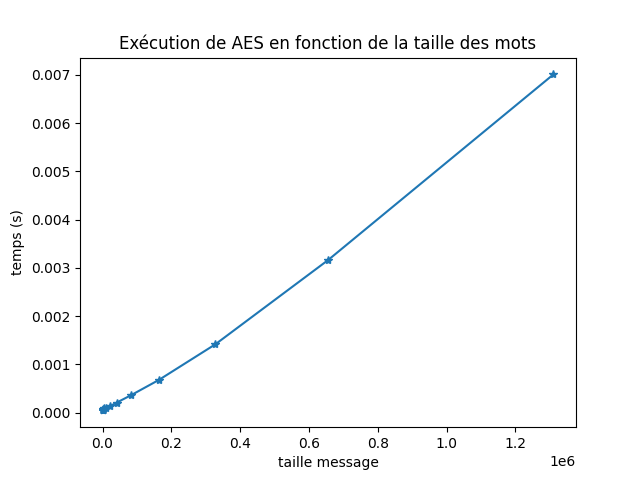
\includegraphics[scale=0.5]{graphe_aes.png}
    \end{center}
\end{minipage}
\end{frame}

\section{Tentative de conservation de l'intégrité des communications}
\begin{frame}{Problème de l'Homme du milieux}
\begin{figure}[H]
  \centering
  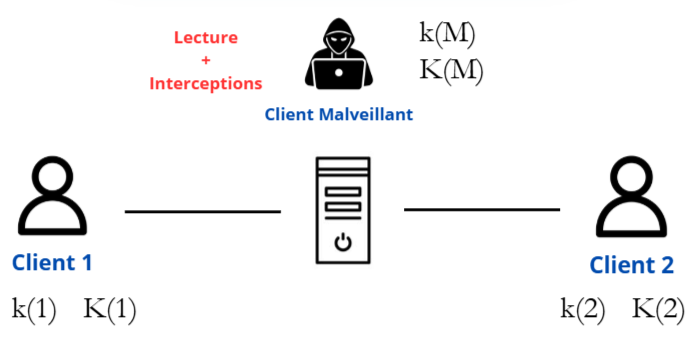
\includegraphics[scale=0.5]{mitm_1.png}
  \caption{Le client malveillant crée ses propres clés $k(M)$ et $K(M)$}
  \label{fig:p_mitm_1}
\end{figure}
\end{frame}

\begin{frame}{Problème de l'Homme du milieux}
\begin{figure}[H]
  \centering
  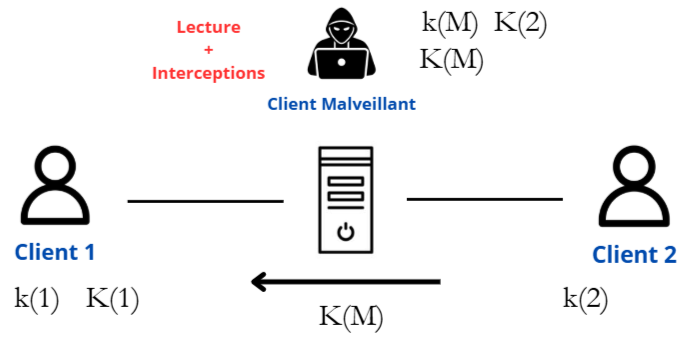
\includegraphics[scale=0.5]{mitm_2.png}
  \caption{Puis il échange $K(2)$ avec $K(M)$ lors de l'envoi de $K(2)$}
  \label{fig:p_mitm_2}
\end{figure}
\end{frame}

\begin{frame}{Problème de l'Homme du milieux}
\begin{figure}[H]
  \centering
  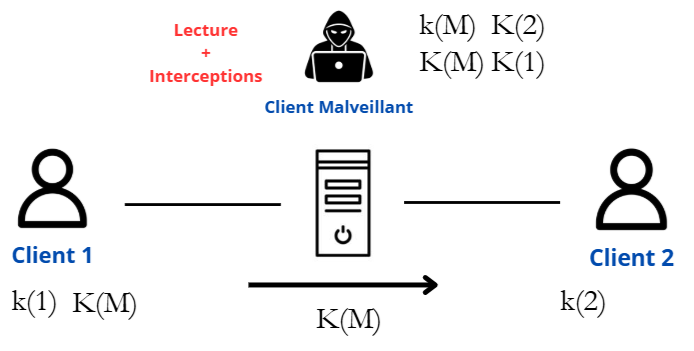
\includegraphics[scale=0.5]{mitm_3.png}
  \caption{Et il échange $K(1)$ avec $K(M)$ lors de l'envoi de $K(1)$}
  \label{fig:p_mitm_3}
\end{figure}
\end{frame}

\begin{frame}{Problème de l'Homme du milieux}
\begin{figure}[H]
  \centering
  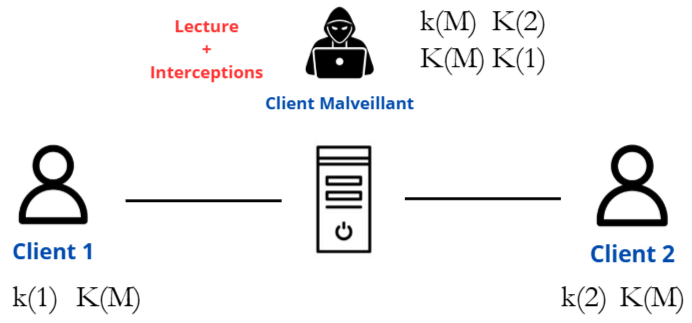
\includegraphics[scale=0.5]{mitm_4.png}
  \caption{Le client malveillant peut donc lire tous les messages échangés}
  \label{fig:p_mitm_4}
\end{figure}
\end{frame}

\begin{frame}{Protocole SAS (Short Authenticated Strings)}
\begin{figure}[H]
  \centering
  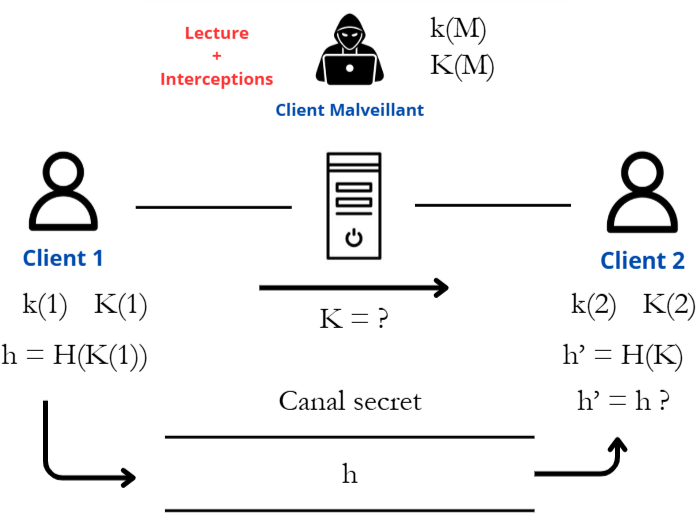
\includegraphics[scale=0.5]{sha_1.png}
  \label{fig:p_sas_1}
\end{figure}
\end{frame}

\begin{frame}{Test pratique}
\begin{figure}[H]
  \centering
  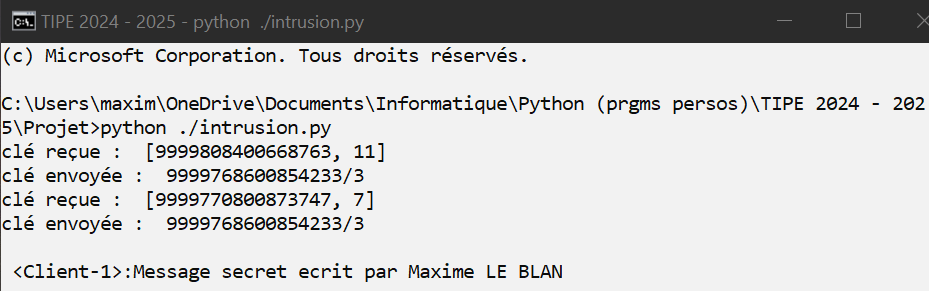
\includegraphics[scale=0.36]{cmd_sha256_1.png}
  \label{fig:cmd_sha256_1}
  \caption{Interface du client malveillant après interception des clés}
  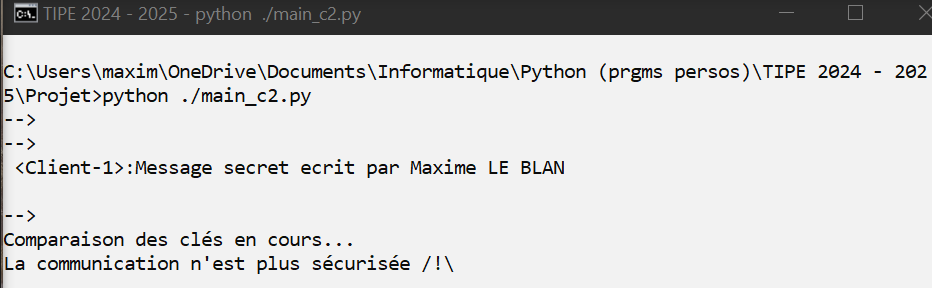
\includegraphics[scale=0.36]{cmd_sha256_2.png}
  \label{fig:cmd_sha256_2}
  \caption{Utilisation du canal secret par le client 1}
\end{figure}
\end{frame}

\begin{frame}{Conclusion}
    \begin{itemize}
        \item Implémentation parallèlisée d'un réseau
        \item Implémentation d'un modèle efficace résistant à la lecture intrusive des données
    \end{itemize}
    \underline{Problèmes :}
    \begin{itemize}
        \item Implémentation du canal secret peu sécurisée et très simplifiée
        \item L'intrusion du client malveillant dans la communication bloque tout échange sécurisé de données
    \end{itemize}
    \underline{Pistes de réflexion :}
    \begin{itemize}
        \item Chercher une alternative au protocole SAS : utilisation de certificats pour l'authentification
    \end{itemize}
\end{frame}

\begin{frame}{Annexe - Preuve déchiffrement RSA}
    \begin{itemize}
        \item Soient $c, m \in \mathbb{N}$, $p, q \in \mathbb{P}$ $(p \neq q)$ et $e,d \in \mathbb{N}$ tel que \newline $ed \equiv 1 \pmod{(p-1)(q-1)}$. Posons $n = p\times q$
        \item Comme $c \equiv m^e \pmod{n}$, alors
        $c^d \equiv m^{ed} \pmod{n}$
        \item De plus, $ed \equiv 1 \pmod{(p-1)(q-1)}$ \newline
        $\Rightarrow \exists k \in \mathbb{N}, ed = 1 + k(p-1)(q-1)$ \newline
        Donc  $c^d \equiv m^{1 + k(p-1)(q-1)} \pmod{n}$
    \end{itemize}
\end{frame}

\begin{frame}{Annexe - Preuve déchiffrement RSA}
    \begin{itemize}
        \item Par conséquent :
        \begin{itemize}
            \item Si $m$ n'est pas un multiple de $p$,  d'après le Petit théorème de Fermat, $m^{p-1}\equiv 1 \pmod{p}$ \newline $\Rightarrow m^{ed} \equiv m^{1 + k(p-1)(q-1)} \equiv m \times (m^{p-1})^{k(q-1)} \pmod{p}$ \newline $\Rightarrow m^{ed} \equiv m \pmod{p}$
            \item Si $m$ est un multiple de $p$, alors $m^{ed} \equiv 0 \pmod{p} \newline \Rightarrow m^{ed} \equiv m \pmod{p}$ 
        \end{itemize}
        Donc $m^{ed} \equiv m \pmod{p}$ et de même, $m^{ed} \equiv m \pmod{q}$
        \item $p$ et $q$ étant premiers, on a donc : \newline
        $m^{ed}-m \equiv 0 \pmod{pq} \newline \Rightarrow m^{ed} \equiv m \pmod{n} \newline \Rightarrow c^d \equiv m \pmod{n}$
    \end{itemize}
\end{frame}

\begin{frame}{Annexe - Fonction de hachage idéale}
    \underline{Propriétés :}
    \begin{itemize}
        \item déterministe
        \item fonction de hachage avec une complexité amortie en $O(1)$
        \item résistance à la préimage : impossibilité, pour une valeur de hachage donnée, de construire un message ayant cette valeur
        \item résistance à la seconde préimage : impossibilité de trouver un second message ayant la même valeur de hachage qu'un message donné
        \item résistance aux collisions
        \item modifier légèrement un message modifie considérablement la valeur de hachage
    \end{itemize}
\end{frame}

\begin{frame}{Annexe - Modules utilisés}
\lstinputlisting{modules.py}
\end{frame}

\begin{frame}{Annexe - algos\_chiffrement.py}
\lstinputlisting{algos_1.py}
\end{frame}

\begin{frame}{Annexe - algos\_chiffrement.py}
\lstinputlisting{algos_2.py}
\end{frame}

\begin{frame}{Annexe - algos\_chiffrement.py}
\lstinputlisting{algos_3.py}
\end{frame}

\begin{frame}{Annexe - algos\_chiffrement.py}
\lstinputlisting{algos_4.py}
\end{frame}

\begin{frame}{Annexe - algos\_chiffrement.py}
\lstinputlisting{algos_5.py}
\end{frame}

\begin{frame}{Annexe - algos\_chiffrement.py}
\lstinputlisting{algos_6.py}
\end{frame}

\begin{frame}{Annexe - algos\_chiffrement.py}
\lstinputlisting{algos_7.py}
\end{frame}

\begin{frame}{Annexe - algos\_chiffrement.py}
\lstinputlisting{algos_8.py}
\end{frame}

\begin{frame}{Annexe - algos\_chiffrement.py}
\lstinputlisting{algos_9.py}
\end{frame}

\begin{frame}{Annexe - algos\_chiffrement.py}
\lstinputlisting{algos_10.py}
\end{frame}

\begin{frame}{Annexe - algos\_chiffrement.py}
\lstinputlisting{algos_11.py}
\end{frame}

\begin{frame}{Annexe - algos\_chiffrement.py}
\lstinputlisting{algos_12.py}
\end{frame}

\begin{frame}{Annexe - serveur.py}
\lstinputlisting{serveur_1.py}
\end{frame}

\begin{frame}{Annexe - serveur.py}
\lstinputlisting{serveur_2.py}
\end{frame}

\begin{frame}{Annexe - serveur.py}
\lstinputlisting{serveur_3.py}
\end{frame}

\begin{frame}{Annexe - serveur.py}
\lstinputlisting{serveur_4.py}
\end{frame}

\begin{frame}{Annexe - serveur.py}
\lstinputlisting{serveur_5.py}
\end{frame}

\begin{frame}{Annexe - serveur.py}
\lstinputlisting{serveur_6.py}
\end{frame}

\begin{frame}{Annexe - client.py}
\lstinputlisting{client_1.py}
\end{frame}

\begin{frame}{Annexe - client.py}
\lstinputlisting{client_2.py}
\end{frame}

\begin{frame}{Annexe - client.py}
\lstinputlisting{client_3.py}
\end{frame}

\begin{frame}{Annexe - client.py}
\lstinputlisting{client_4.py}
\end{frame}

\begin{frame}{Annexe - client.py}
\lstinputlisting{client_5.py}
\end{frame}

\begin{frame}{Annexe - client.py}
\lstinputlisting{client_6.py}
\end{frame}

\begin{frame}{Annexe - client.py}
\lstinputlisting{client_7.py}
\end{frame}

\begin{frame}{Annexe - client.py}
\lstinputlisting{client_8.py}
\end{frame}

\begin{frame}{Annexe - client.py}
\lstinputlisting{client_9.py}
\end{frame}

\begin{frame}{Annexe - client.py}
\lstinputlisting{client_10.py}
\end{frame}

\begin{frame}{Annexe - client.py}
\lstinputlisting{client_11.py}
\end{frame}

\begin{frame}{Annexe - client.py}
\lstinputlisting{client_12.py}
\end{frame}

\begin{frame}{Annexe - client.py}
\lstinputlisting{client_13.py}
\end{frame}

\begin{frame}{Annexe - client.py}
\lstinputlisting{client_14.py}
\end{frame}

\begin{frame}{Annexe - fonctions\_utiles.py}
\lstinputlisting{fu_1.py}
\end{frame}

\begin{frame}{Annexe - fonctions\_utiles.py}
\lstinputlisting{fu_2.py}
\end{frame}

\begin{frame}{Annexe - fonctions\_utiles.py}
\lstinputlisting{fu_3.py}
\end{frame}

\begin{frame}{Annexe - fonctions\_utiles.py}
\lstinputlisting{fu_4.py}
\end{frame}

\begin{frame}{Annexe - fonctions\_utiles.py}
\lstinputlisting{fu_5.py}
\end{frame}

\begin{frame}{Annexe - fonctions\_utiles.py}
\lstinputlisting{fu_6.py}
\end{frame}

\begin{frame}{Annexe - fonctions\_utiles.py}
\lstinputlisting{fu_7.py}
\end{frame}

\begin{frame}{Annexe - fonctions\_utiles.py}
\lstinputlisting{fu_8.py}
\end{frame}

\begin{frame}{Annexe - fonctions\_utiles.py}
\lstinputlisting{fu_9.py}
\end{frame}

\begin{frame}{Annexe - fonctions\_utiles.py}
\lstinputlisting{fu_10.py}
\end{frame}

\end{document}
